\subsection{Class Diagram}

\begin{figure}[H]
    \centering
    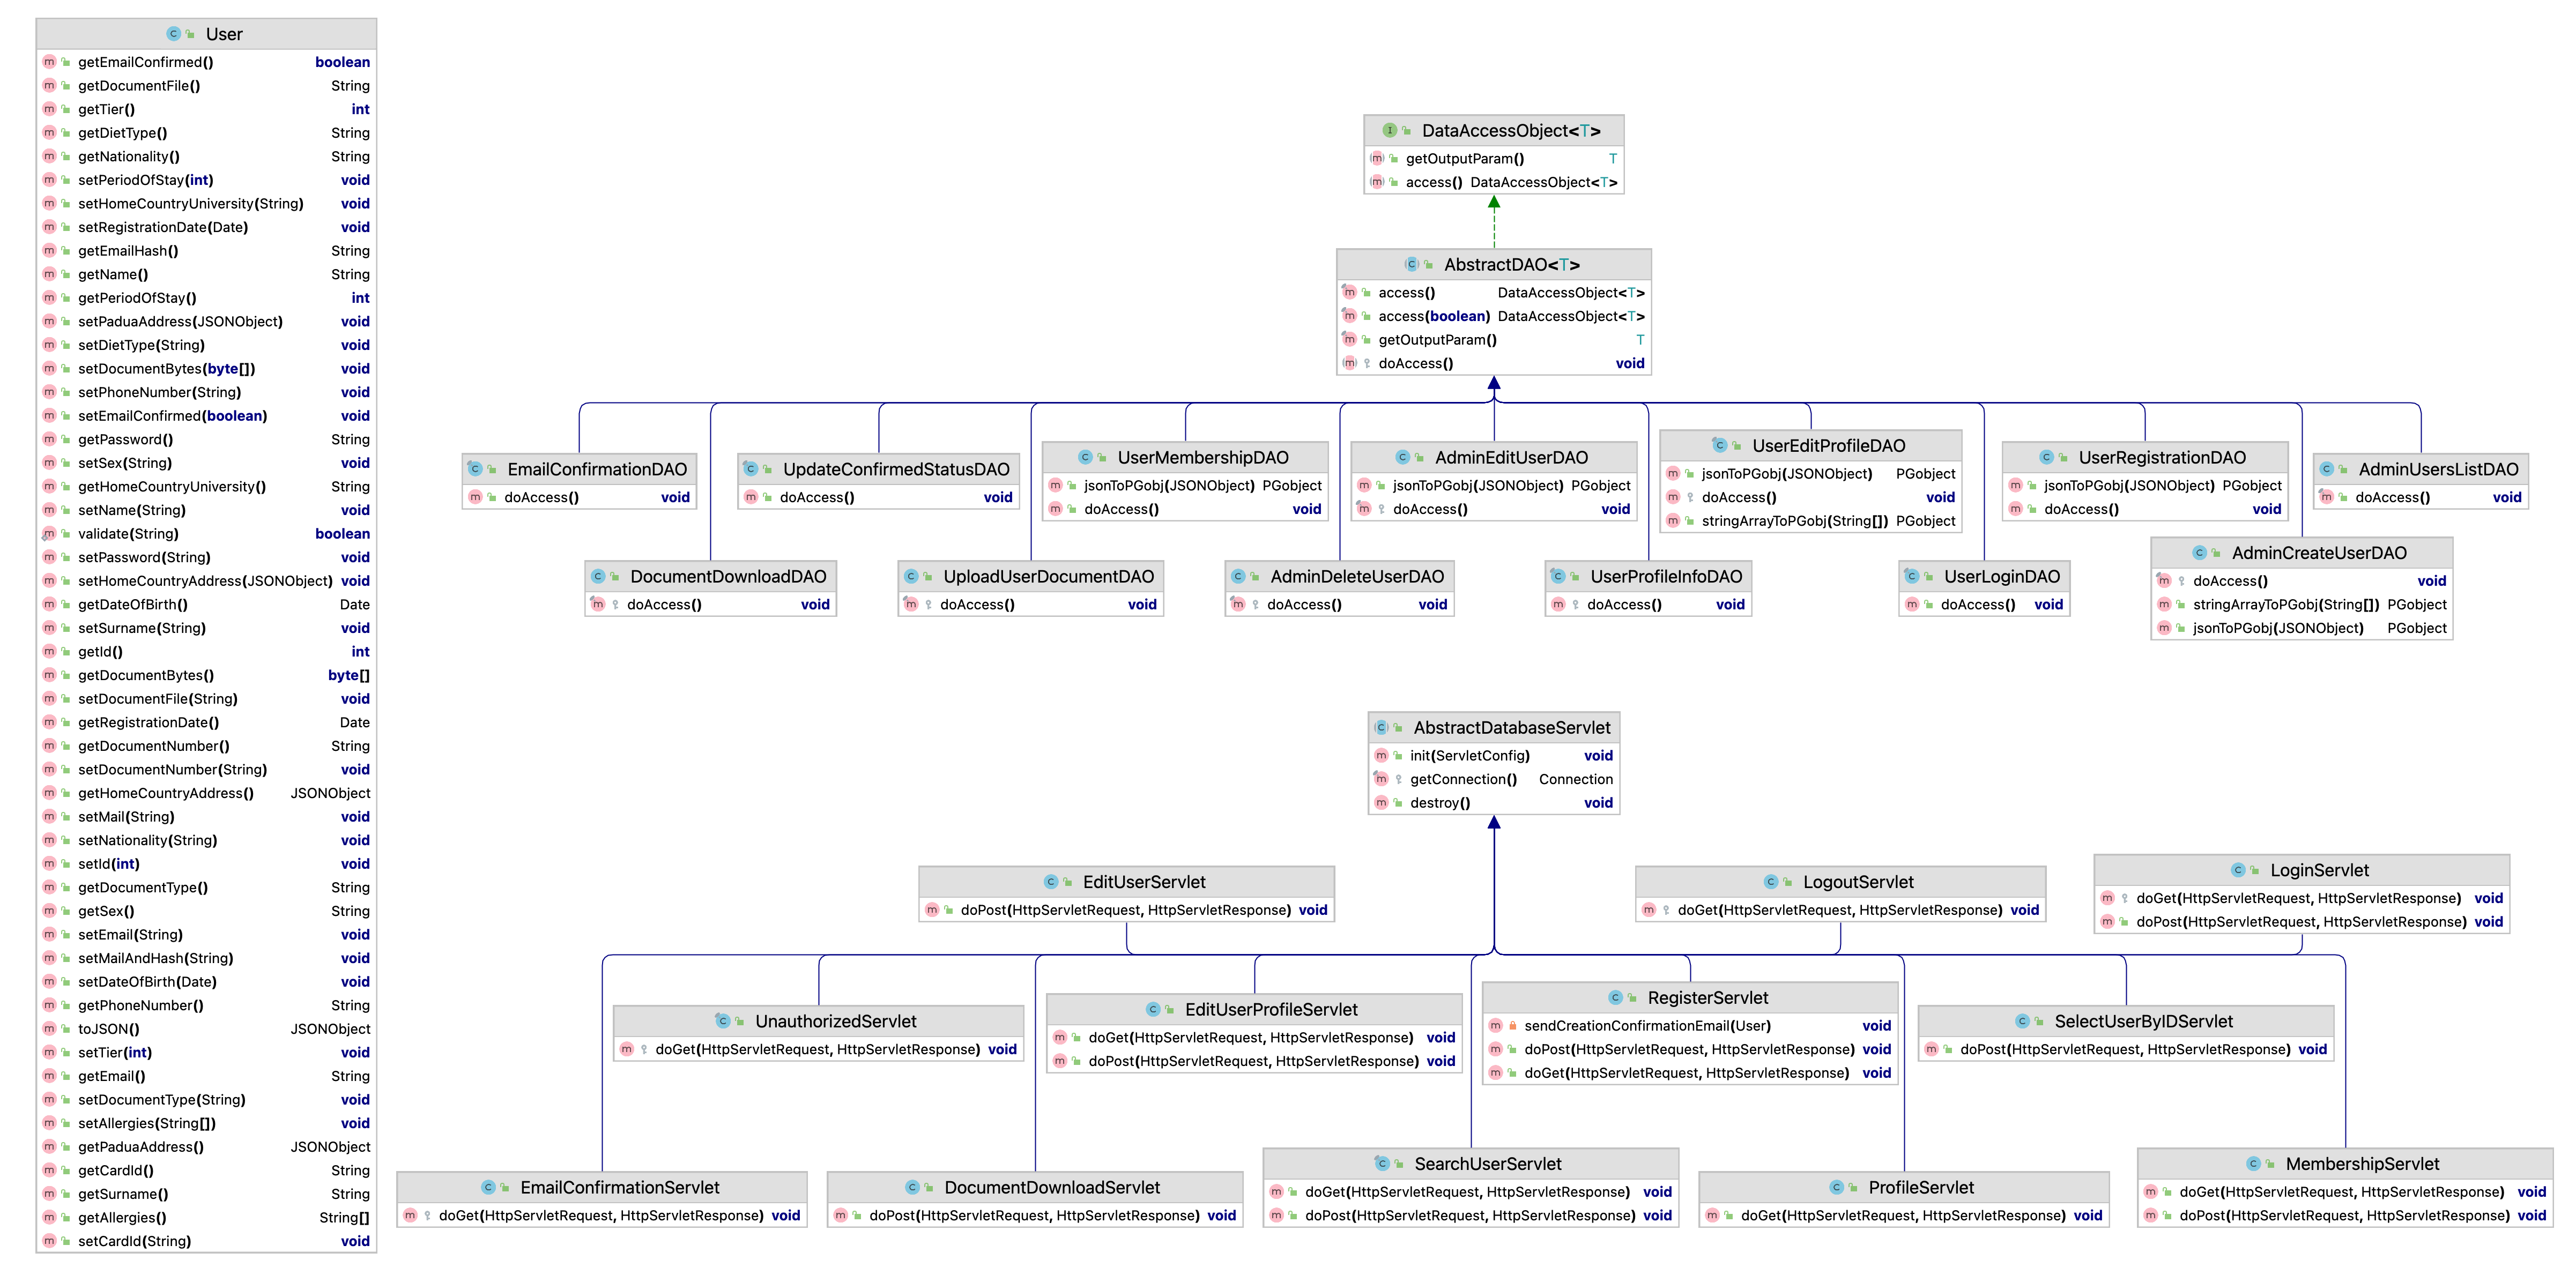
\includegraphics[width=1\textwidth]{images/classUser.png}
    \caption{User class diagram}
    \label{fig:user class diagram}
\end{figure}

\begin{figure}[H]
    \centering
    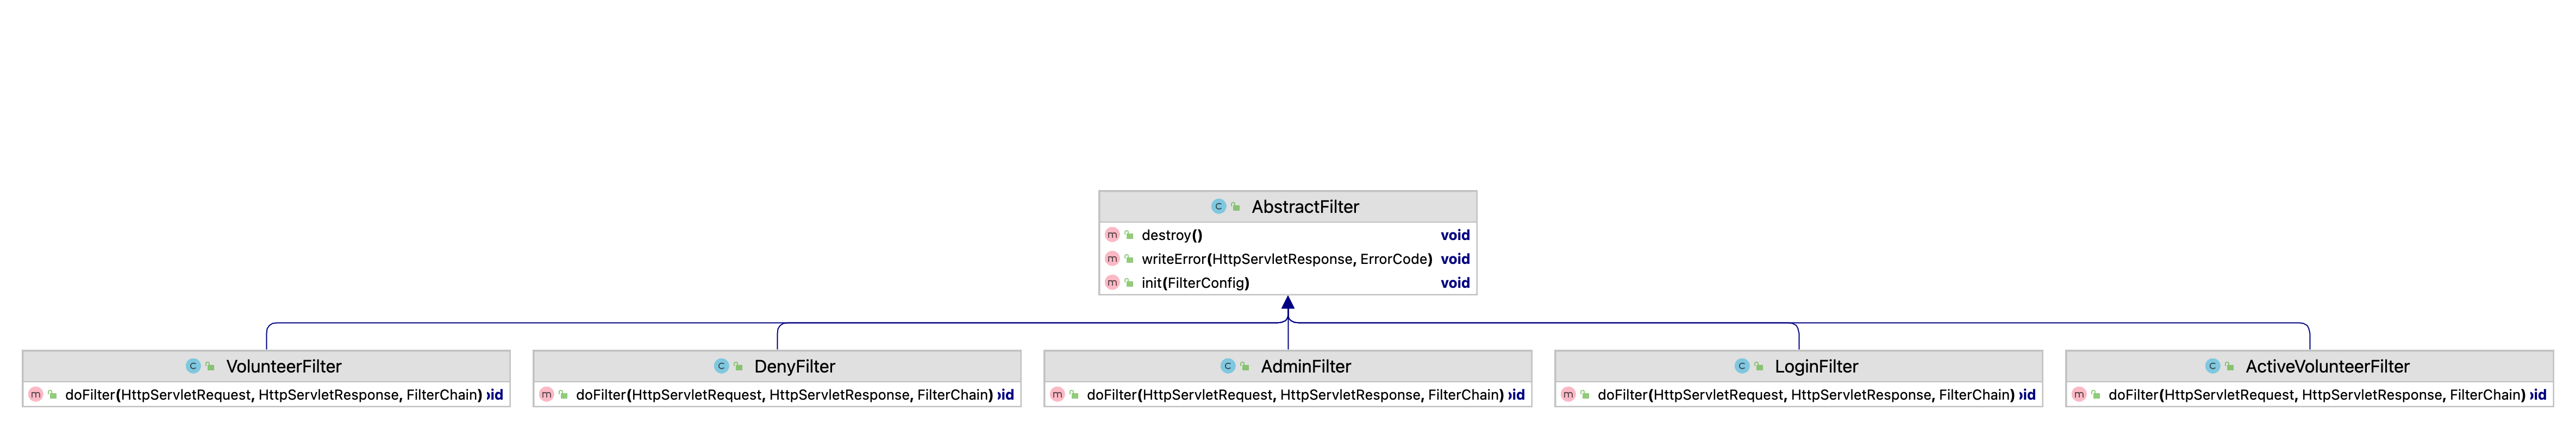
\includegraphics[width=1\textwidth]{images/classFilterDiagram.png}
    \caption{Filters class diagram}
    \label{fig:filters}
\end{figure}

\begin{figure}[H]
    \centering
    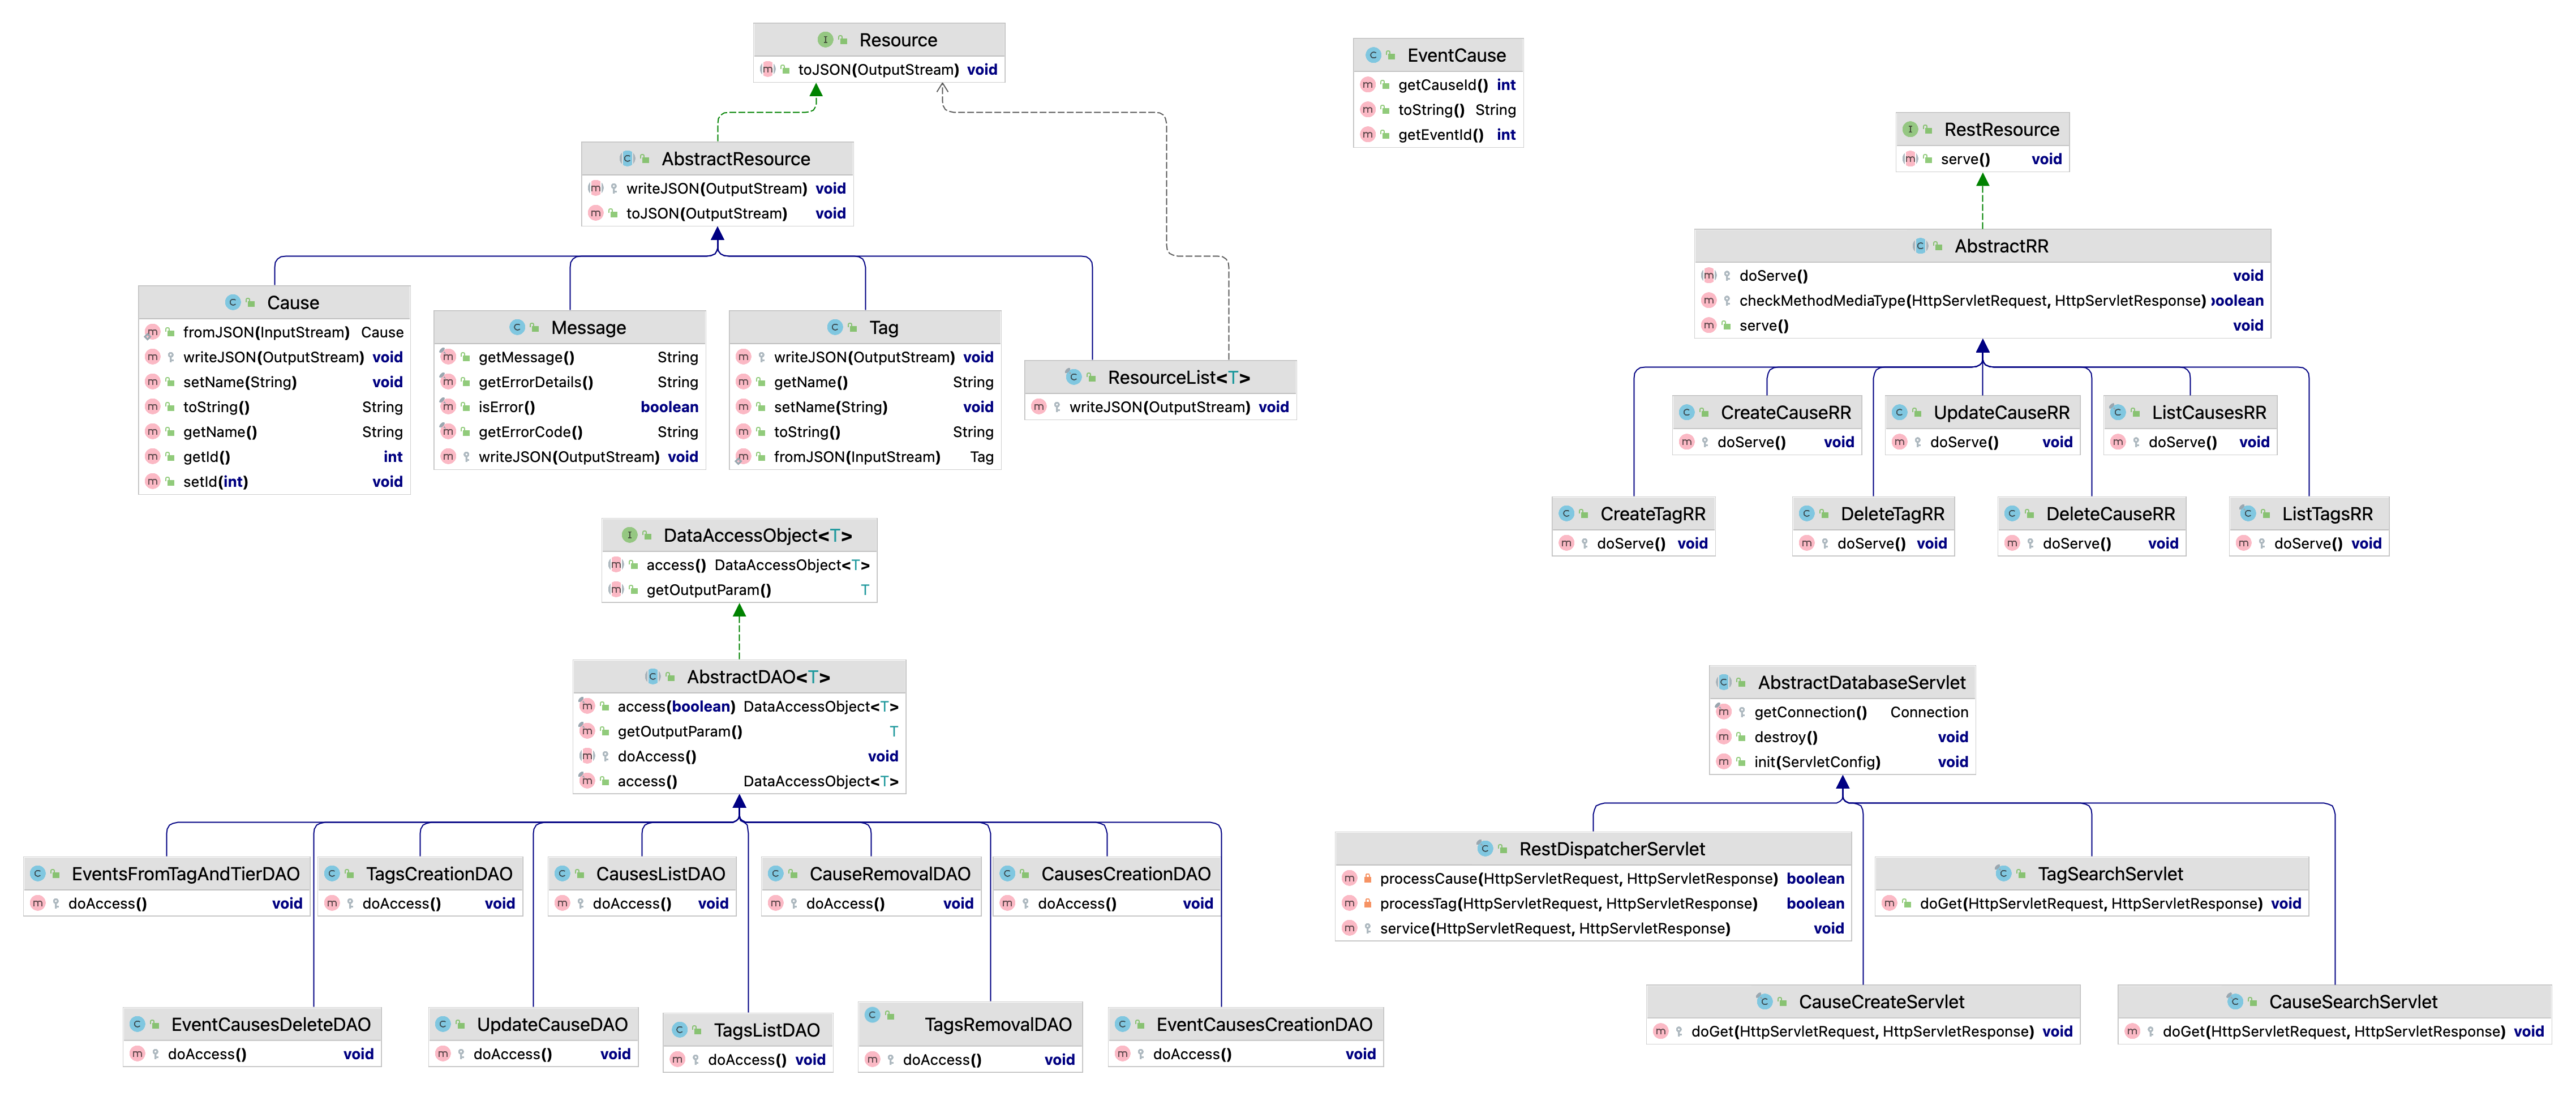
\includegraphics[width=1\textwidth]{images/classRest.png}
    \caption{Rest class diagram}
    \label{fig:rest}
\end{figure}

\begin{figure}[H]
    \centering
    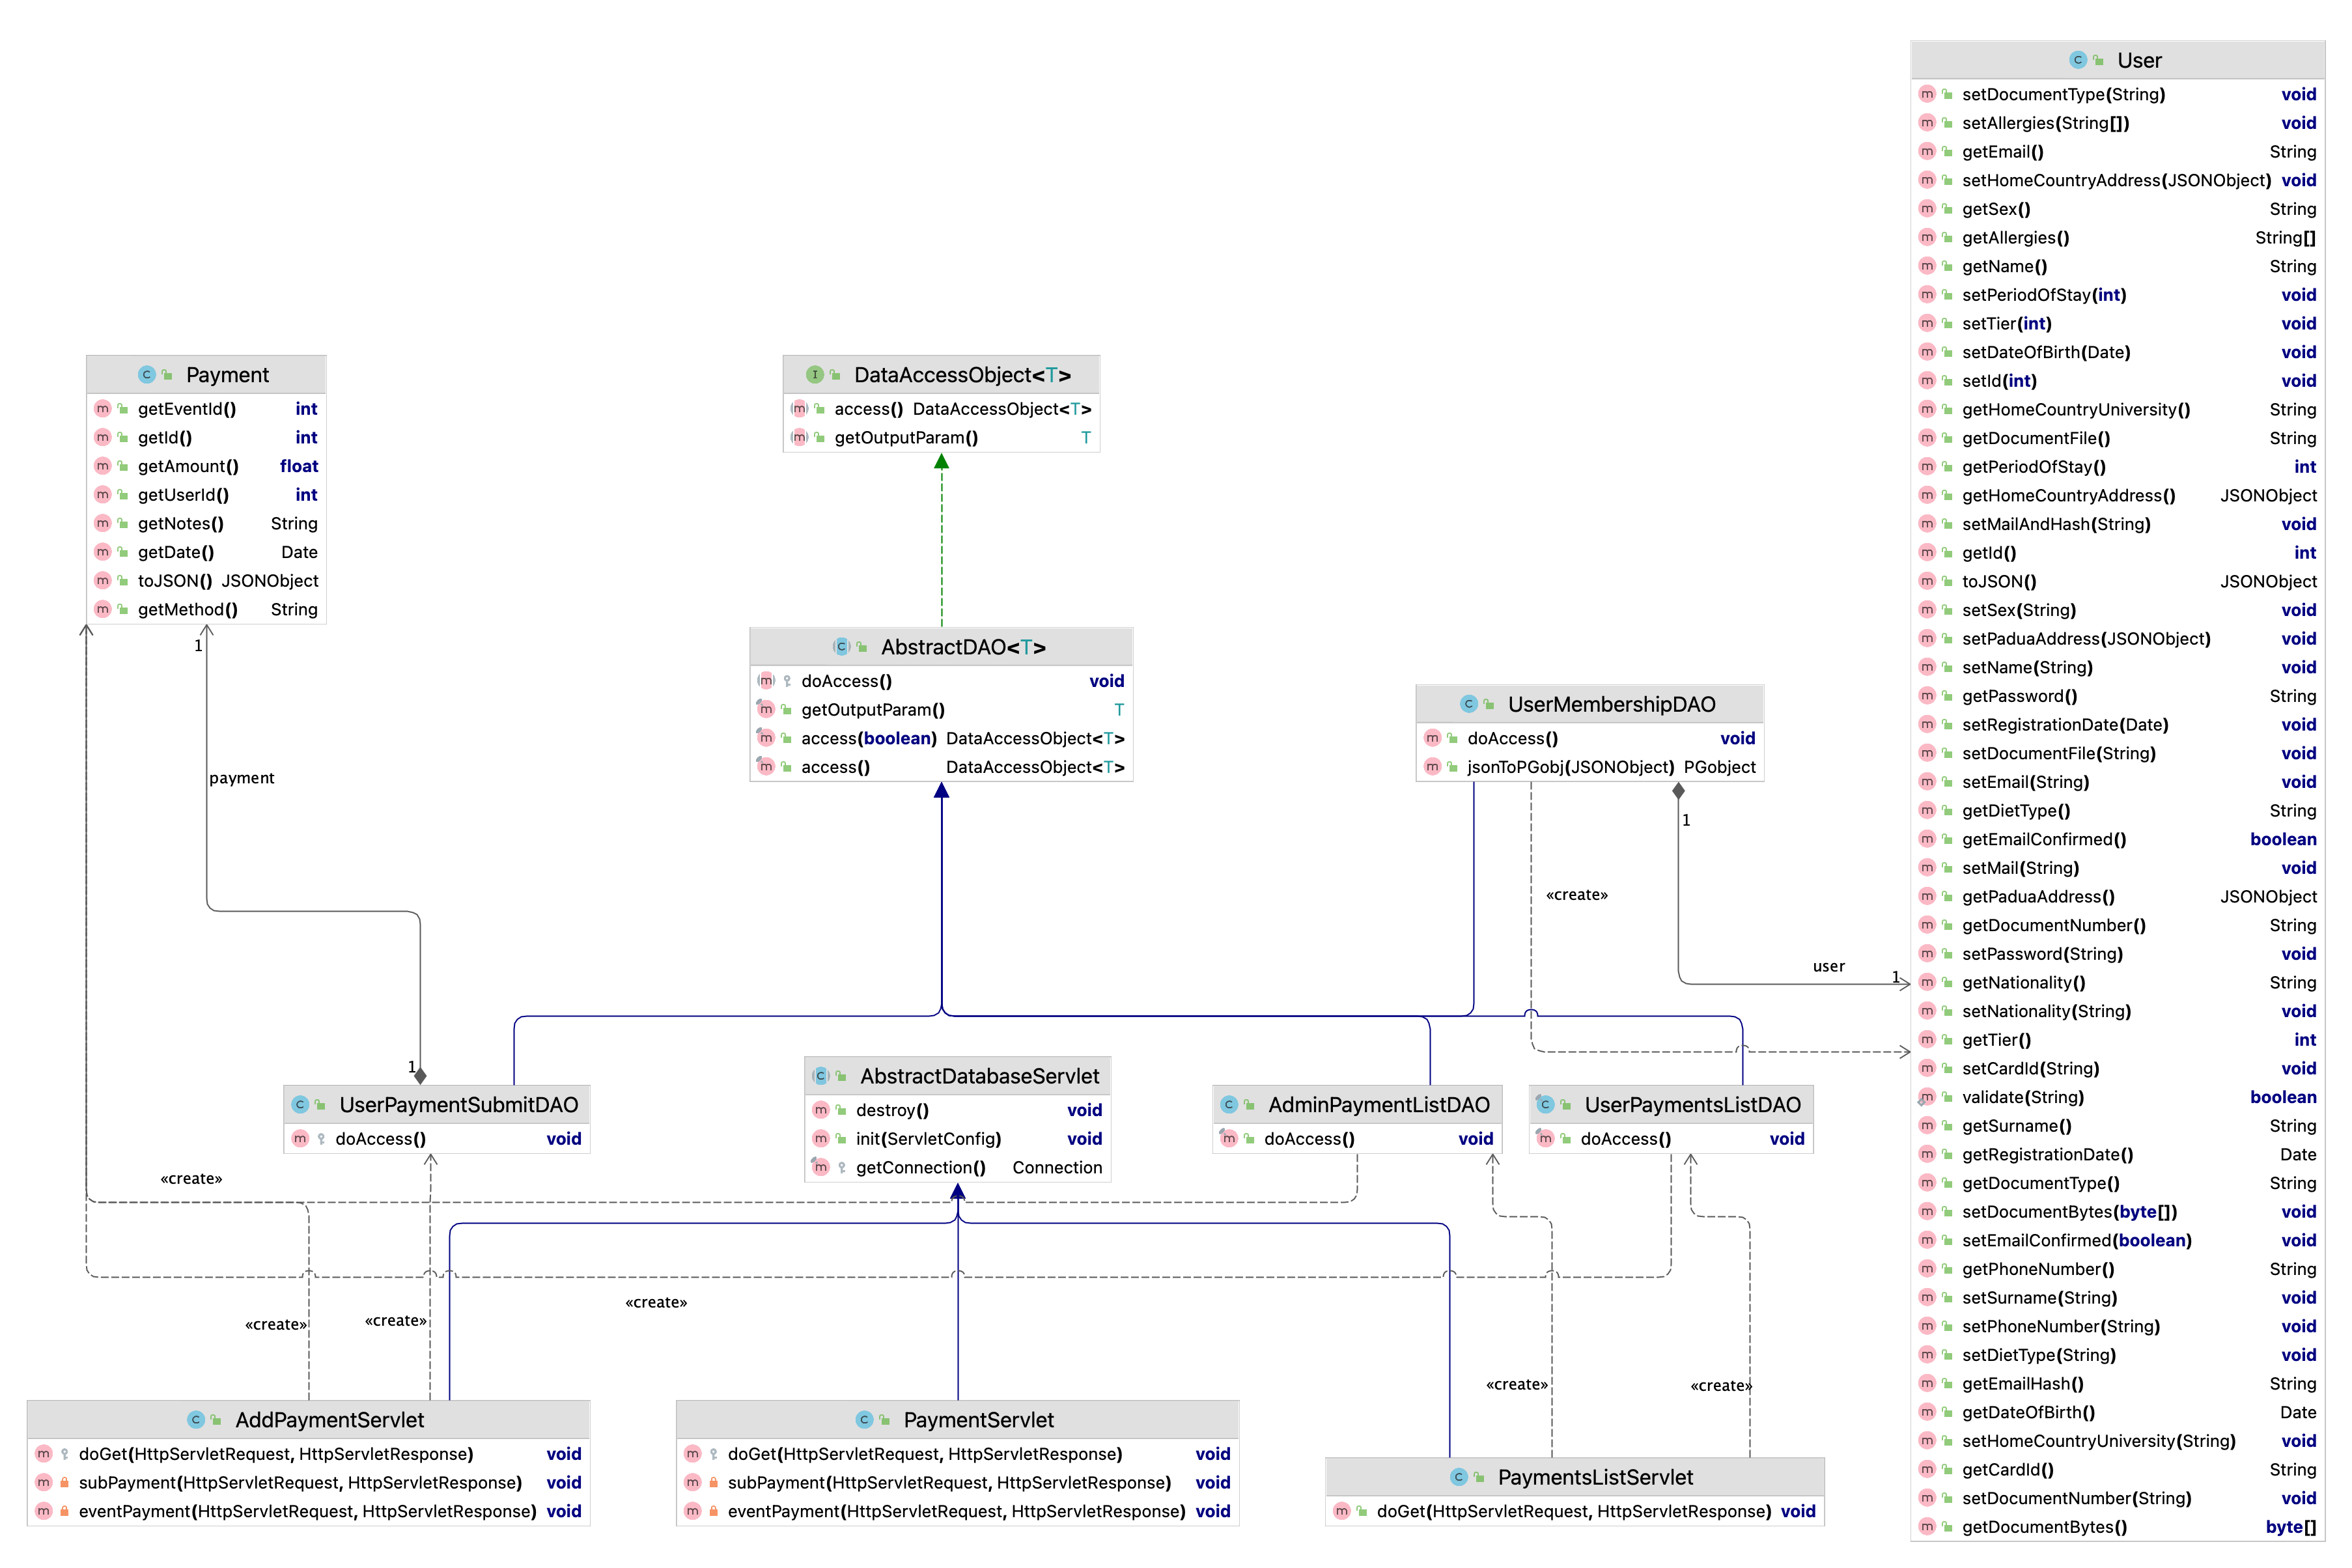
\includegraphics[width=1\textwidth]{images/classPaymentUser.png}
    \caption{Payment class diagram}
    \label{fig:payment}
\end{figure}

To make it as clear as possible, we have divided the class diagram into 3 sections (which do not represent all the classes in the application). The sections were selected based on the entities presented in the data layer.\\
All twenty-seven servlets that make up the application extend AbstractDatabaseServlet.The role of the abstract servlet is to provide a template for managing the connection pool to the database and extends HttpServlet, thus making all servlets required to override at least one of the following methods: doGet, doPost, doPut, doDelete, getServletInfo, init and destroy.\\
The servlets can access the database through specific DAOs, which separate the application logic from the database access logic, acting as an intermediary between the application and the database.\\
Regarding filters \ref{fig:filters}, they extend the abstract class AbstractFilter, which defines methods for initializing, processing, and destroying requests and responses in a web application.